\section{Introduction}
In this chapter, in section \ref{sec:crud} will be discussed the tests used to develop the two Kundera extensions.
In section \ref{sec:performance} will be described the YCSB framework that we have used to test the performance of the developed extensions with respect to the low level API.
Finally in section \ref{sec:data} we present the application developed to test the data synchronization capabilities of CPIM while persisting data through the Datastore Kundera extension. 

\section{Test CRUD operations}
\label{sec:crud}
The Kundera extensions development, due to the lack of information both in the documentation and from the community, has been approached in a test driven way.
The first step was then writing the required JUnit tests for the features we have planned to support.

\newparagraph We primarily want to achieve code portability of model classes, this should be exploited by the usage of the JPA interface but, as stated in chapter \ref{chap:ps}, there were problems in the old NoSQL service implementation relatively to this point.
Secondary we want to be sure that while entities are persisted in the underlying NoSQL database, they can be restored without any loss of information and thus the mapping between entities and the NoSQL database data model behave correctly in both verses.
Hence test the extensions cannot be done directly by testing single methods behavior inside the extensions code, this will for sure test the correctness of the operations but, since Kundera clients are not obliged to follow a rigid structure for their code in the implementation of the required interfaces, tests written for a client are not guaranteed to run correctly for another one. 

\noindent The approach we adopted was to define a single test suite, that will test each one of the feature we planned to support, by interacting directly with Kundera through the JPA interface. This make us able to use the same tests independently of the specific extension and thus testing the correctness of CRUD operations through the JPA interface and the portability of the code by means of tests portability.

\noindent Those tests have been primarily used to test the extensions during the development phase but they have also been executed on the remote databases instances by connecting to them through the network from the development machine. This test has been made to guarantee the correct functioning of the two extensions on real databases instance since tests runned locally are executed  against emulators of real storages.

\subsection{Tests structure}
Tests are composed by the entities, annotated with the JPA annotations, and a test class for each feature.
There are 20 defined entities that includes:
\begin{itemize}
\item simple entities related with the JPA relationships annotations, used to test relationships among entities;
\item embeddable entities and specific entities that uses those embeddable entities as data types, both types used to test the embedded feature;
\item entities with enum fields, used to test the enum fields support;
\item entities declared with different data types for the primary key identifier, used to test ids auto-generation and user-defined ids validation.
\end{itemize}

\noindent The test classes developed for testing the correctness of relationships are:
\begin{itemize}
\item \texttt{MTMTest}, to test the \textit{Many to Many} relationship type;
\item \texttt{MTOTest}, to test the \textit{Many to One} relationship type;
\item \texttt{OTMTest}, to test the \textit{One to Many} relationship type;
\item \texttt{OTOTest}, to test the \textit{One to One} relationship type;
\end{itemize}
\noindent All of those test classes implements two different methods: \texttt{testCRUD()}, that test the relationship by interacting with the method of the \texttt{EntityManager} interface, and \texttt{testQuery()}, that test the relationships by reading, updating and deleting entities through JPQL queries.

\newparagraph The remaining tests classes are:
\begin{itemize}
\item \texttt{ElementCollectionTest}, that tests the JPA feature for persisting list of entities within another one;
\item \texttt{EmbeddedTest}, that tests the JPA feature of persisting user-defined data-types as field of entities;
\item \texttt{EnumeratedTest}, that tests the JPA feature of persisting enum fields;
\item \texttt{QueryTest}, that tests the execution of various \textit{SELECT} queries and the support for the various JPQL clauses in queries.
\end{itemize}

\section{Performance tests}
\label{sec:performance}
We wanted to test the overhead of the developed Kundera extensions with respect to direct use of low-level API. To test those kind of performance in terms of throughput and latency of the read and write operations, we have used Yahoo Cloud Serving Benchmark.
We choose this approach since it was already used by Kundera developers to estimate the overhead that Kundera adds to the low-level API versions of its clients. Hence by using the same method we are able to compare our results to the ones of Kundera.

\subsection{Yahoo Cloud Serving Benchmark}
Yahoo Cloud Serving Benchmark (YCSB) is a framework with the general goal of facilitating performance comparisons of the new generations o cloud serving systems \cite{paper:ycsb}.

\noindent YCSB provides the facility to benchmark various NoSQL database systems such Cassandra, DynamoDB, Voldemort, MongoDB and many others.
The key feature of the benchmark system is extensibility, it in facts supports easy definition of new \textit{workloads} and new systems to benchmark.

\begin{figure}[tbh]
  \centering
  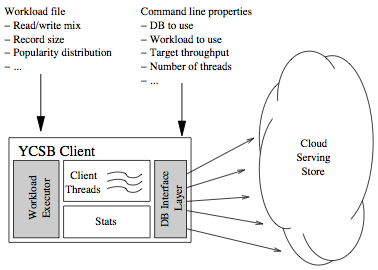
\includegraphics[width=10cm]{images/ycsb_architecture}
  \caption{YCSB architecture \cite{paper:ycsb}}
  \label{fig:ycsb-architecture}
\end{figure} 

\newparagraph The access point to the benchmark framework is the \textit{YCSB Client} which is responsible of generating the operations which make up the workload. The workload is then executed by the \textit{Workload executor} that drives multiple client threads which in turn execute a sequential series of operations by making calls to the \textit{database interface layer}.
The workloads are executed in two separate phases:
\begin{enumerate}
\item the \textbf{load phase}, which loads the workload data to the datastore instance;
\item the \textbf{transaction phase}, which execute the workload on the loaded data.
\end{enumerate}
\noindent Each thread rules the rate at which it generate requests ad measure the latency and the throughput of its operation. At the end of the benchmark, the statistics modules aggregates the measurements and build the report.

\subsection{YCSB adapters}
The YCSB Client abstracts from the specific database system under test through the \textit{database interface layer}. This allows YCSB to generate operations like ``read record'' or ``update record'' without having to understand the specific API of the underlying database. The  \textit{database interface layer} is a simple abstract class that provides read, insert, update, delete and scan operations. 
\noindent To create a database adapter the abstract class \texttt{com.yahoo.ycsb.DB} must be extended and the following methods needs to be implemented:
\begin{itemize}
\item \texttt{init()}, which is used to perform any initialization operation such as connecting to the database instance and is called once per thread;
\item \texttt{read(String table, String key, ...)}, which is supposed to read a single record;
\item \texttt{scan(String table, String startkey, int recordcount, ...)}, which is supposed to perform a range scan;
\item \texttt{insert(String table, String key, ...)}, which is supposed to update a single record;
\item \texttt{delete(String table, String key)}, which is supposed to delete a record.
\end{itemize}

\newparagraph To be able to compare the benchmarks result to the Kundera ones, we developed  several YCSB adapters:
\begin{itemize}
\item an adapter for Google Datastore low-level API
\item an adapter for Google Datastore through the developed Kundera extension
\item an adapter for Azure Tables low-level API
\item an adapter for Azure Tables through the developed Kundera extension
\end{itemize}
\noindent Even if the adapters for Hbase were already been developed by Kundera, they have been both re-written. The Kundera client adapter were re-written to be identical to the ones for Google Datastore and Azure Tables; the low-level API version were re-written because the Kundera client for Hbase has been updated to supported the latest version of the software but the YCSB adapter was not.

\subsubsection{Kundera adapters}
For the Kundera version of the adapters the same structure has been kept for all three databases. The \texttt{EntityManagerFactory} is instantiated at the adapter construction since this operation causes Kundera to initialize all its internal structure; an instance of the entity manager is instead created in the \texttt{init} method since the initialization of the \texttt{EntityManager} causes the initialization of the specific Kundera client, in this way each thread will have its own \texttt{EntityManager} with which interact and the same overhead with regards to database connection operation.
Apart from the \texttt{scan} method, which was not implemented, every other operations calls the responsible method on the \texttt{EntityManager}, in the code \ref{code:insert-operation} is shown an example for the insert operation.

\begin{lstlisting}[language=Java, caption=Insert operation of the Azure Tables adapter, label=code:insert-operation]
@Override
public int insert(String table, String key, ...) {
    ...
    try {
        AzureTableUser user = new AzureTableUser(key, nextString(),, ...);
        em.persist(user);
        if (timeToClearEntityManager()) {
            em.clear();
        }
        return OK;
    } catch (Exception e) {
        return ERROR;
    }
}
\end{lstlisting}

\noindent In the code \ref{code:insert-operation} there are two elements that are worth deep explanation. The first thing to notice is that is persisted an instance of \texttt{AzureTableUser} in fact we were not able to persist the entities generated by YCSB because, to be able to persist an entity with the JPA, we need an annotated class which is then listed in the \textit{persistence.xml}. For this reasons three different user class and three different persistence units has been defined:
\begin{itemize}
\item \texttt{AzureTableUser}, which refer to \texttt{kundera\textunderscore azure\textunderscore pu}, the persistence unit with the configuration for Azure Tables;
\item \texttt{DatastoreUser}, which refer to \texttt{kundera\textunderscore datastore\textunderscore pu}, the persistence unit with the configuration for Google Datastore;
\item \texttt{HBaseUser}, which refer to \texttt{kundera\textunderscore hbase\textunderscore pu}, the persistence unit with the configuration for Hbase.
\end{itemize} 
\noindent The second thing to notice is the call to the \texttt{timeToClearEntityManager()} method, which checks, with respect to an internal counter, if has been persisted 500 entities, if this is the case the persistence cache is cleared by calling \texttt{EntityManager.clear()}. If this operation is not performed, entities read can occur within the persistence cache bypassing the request to the underling database. We choose to clear the cache every 500 entities in our workloads of 100.000 entities, to maintains the same proportion with the one used by Kundera in their test in which they clear the entity manager every 5.000 entities on workloads of 1 million operations.

\subsubsection{Low-level API adapters}
Also the adapters for the low-level API version follows the same general structure. The connection to the database is performed, through low-level API in the \texttt{init} method, to have a common behavior with respect to the Kundera adapters; read, insert and delete operations are performed by a call to the low-level API, while the \texttt{scan} method has not been implemented.

\noindent The \texttt{init} method uses the properties defined in the property filesm specified in the execution command of the benchmark, to locate the remote database and instantiate a connection.

\subsection{YCSB tests}
YCSB comes with a core set of workloads, each workloads represents a particular mix of read and write operations and define the total number of operations that should be executed. 
\noindent YCSB benchmarks are executed in two separate phases and each of them generates a report. From the report of the \textit{load} phase, since this phase is responsible of storing the data required to run the workload to the target database, we obtains information about the throughput and the latency for the write operation; from the \textit{transaction} phase we want to obtain information about throughput and latency for the read operation. To do this we run a custom workload composed of 100.000 operations entirely of type read so that the \textit{transaction} phase will generates the statistics we need.
\noindent Defined the adapters and the workload we were able to execute the tests.

\subsubsection{Google Datastore tests}
The tests for Google Datastore has been executed over a remote Datastore instance in an application billed by Politecnico di Milano and configured to accept remote API execution.

\noindent The results of the tests are reported in figure \ref{fig:gae-test-read} for the read operation and in figure \ref{fig:gae-test-write} for the write operation.
 
\begin{figure}[tbh]
  \centering
  \subfloat[Throughput]{
    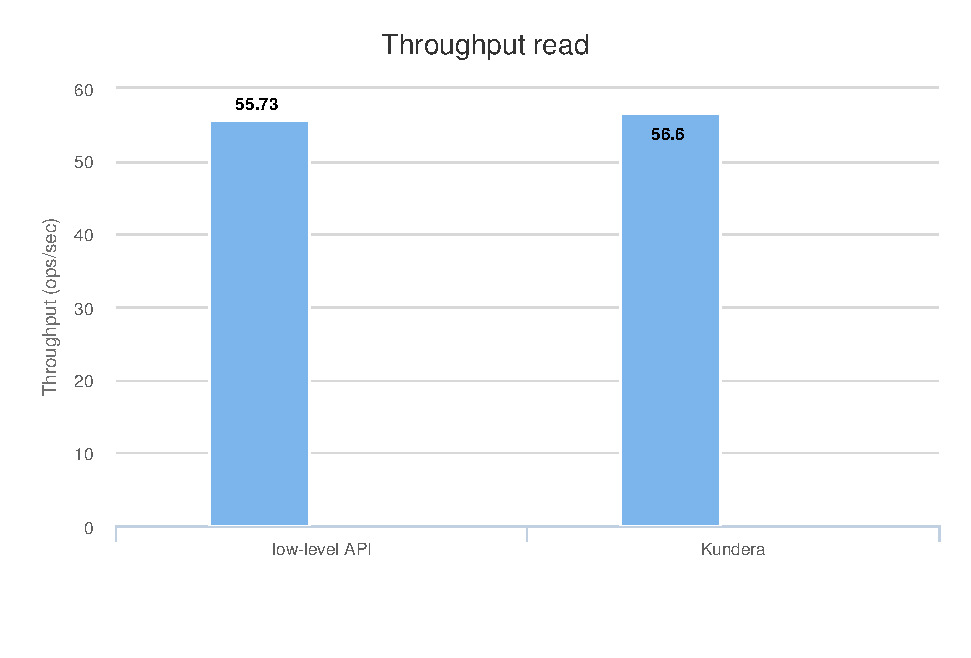
\includegraphics[width=7cm]{images/gae-read-throughput}
  }
  \subfloat[Latency]{
    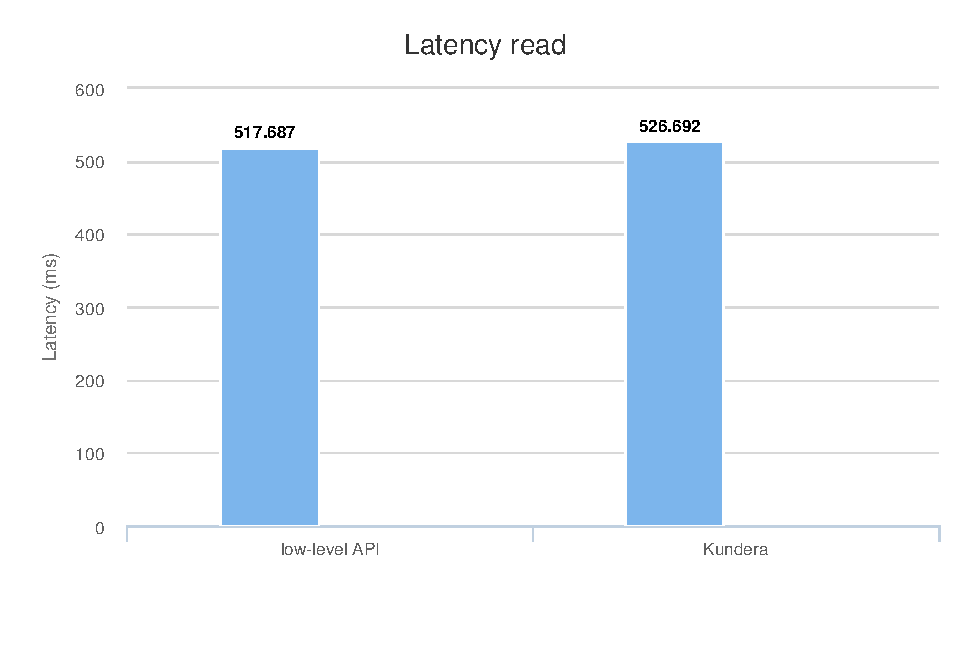
\includegraphics[width=7cm]{images/gae-read-latency}
  }
  \caption{Google Datastore - read operation benchmark results}
  \label{fig:gae-test-read}
\end{figure} 

\begin{figure}[tbh]
  \centering
  \subfloat[Throughput]{
    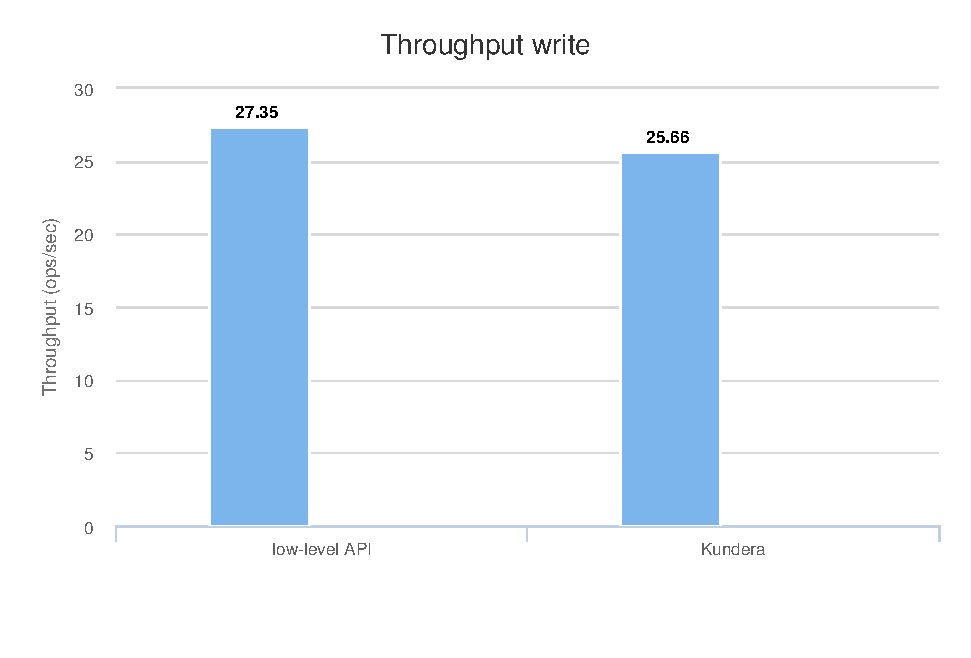
\includegraphics[width=7cm]{images/gae-write-throughput}
  }
  \subfloat[Latency]{
    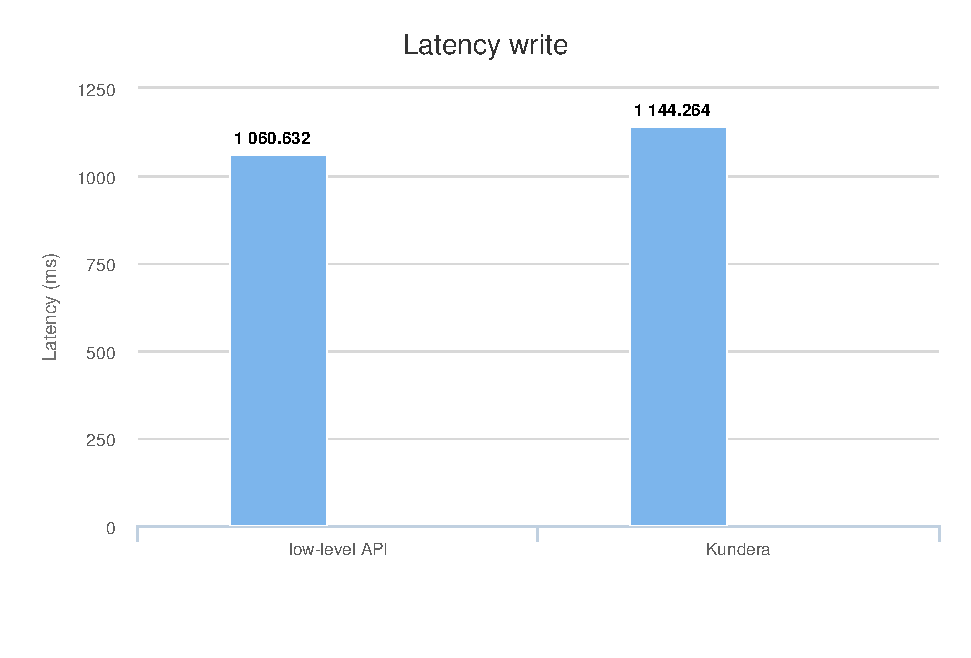
\includegraphics[width=7cm]{images/gae-write-latency}
  }
  \caption{Google Datastore - write operation benchmark results}
  \label{fig:gae-test-write}
\end{figure} 
 
\subsubsection{Azure Tables tests}
The tests for Azure Tables has been executed over a remote storage instance deployed in Azure from the billing account of Politecnico di Milano.

\noindent The results of the tests are reported in figure \ref{fig:azure-test-read} for the read operation and in figure \ref{fig:azure-test-write} for the write operation.
 
\begin{figure}[tbh]
  \centering
  \subfloat[Throughput]{
    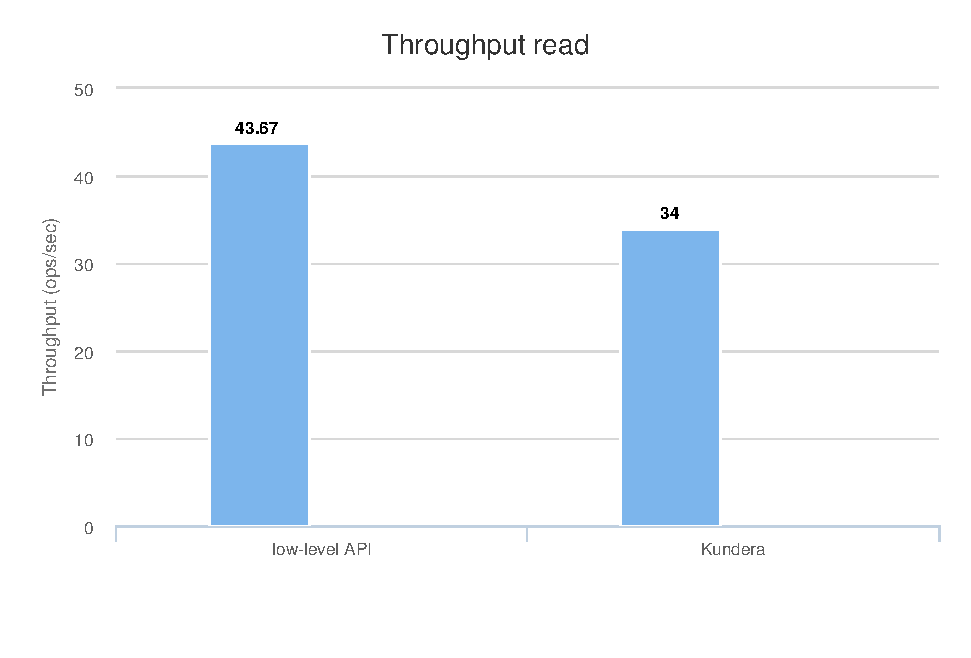
\includegraphics[width=7cm]{images/azure-read-throughput}
  }
  \subfloat[Latency]{
    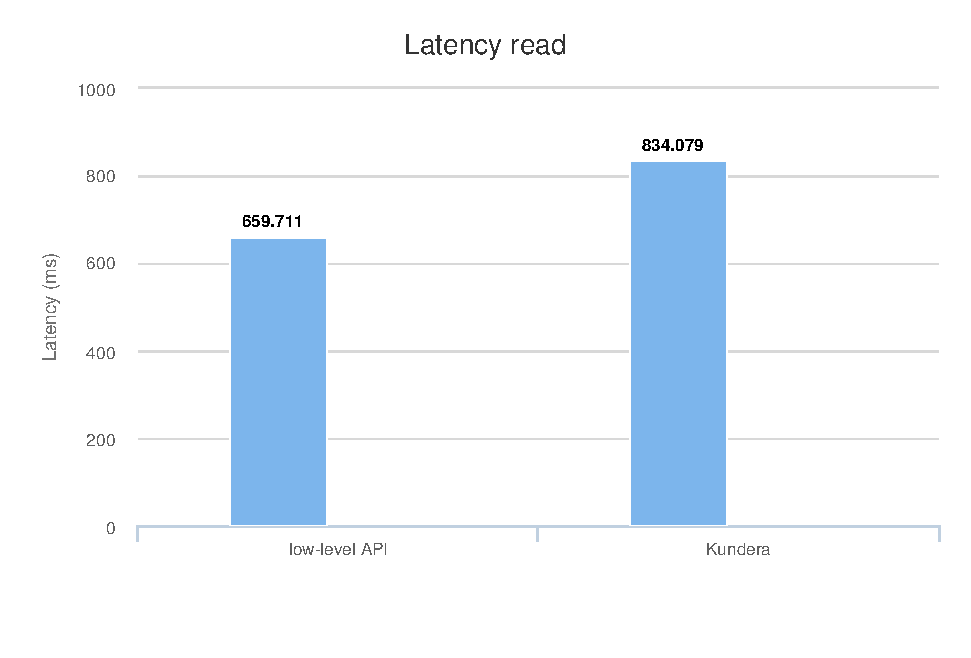
\includegraphics[width=7cm]{images/azure-read-latency}
  }
  \caption{Azure Tables - read operation benchmark results}
  \label{fig:azure-test-read}
\end{figure} 

\begin{figure}[tbh]
  \centering
  \subfloat[Throughput]{
    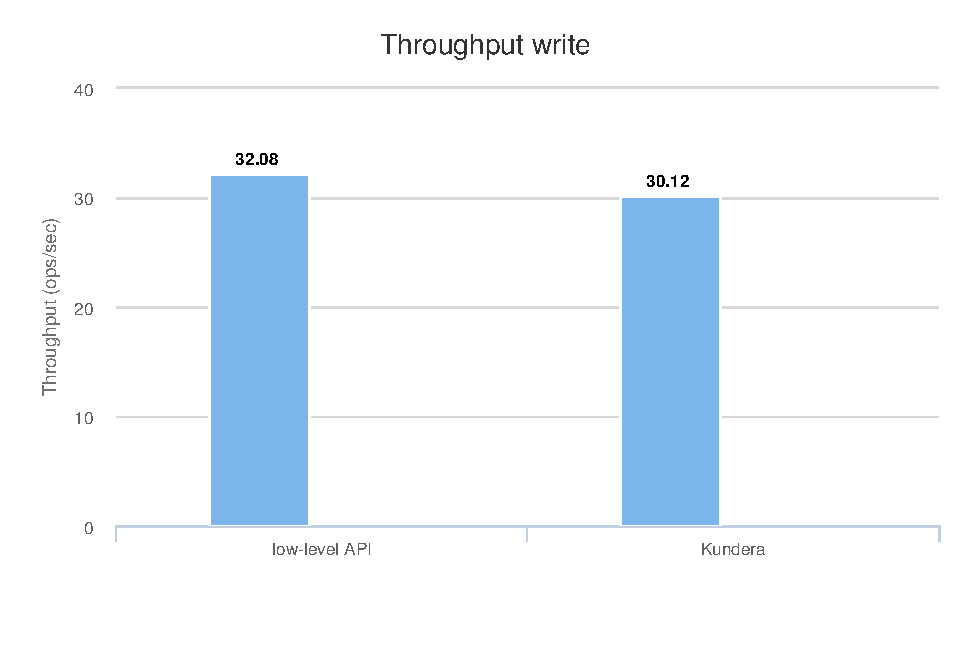
\includegraphics[width=7cm]{images/azure-write-throughput}
  }
  \subfloat[Latency]{
    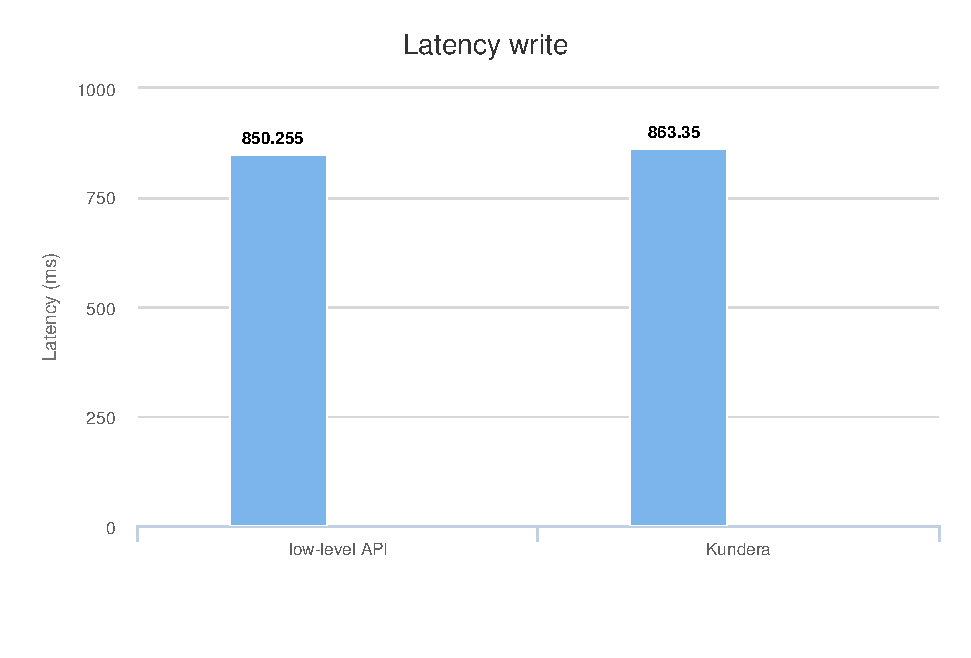
\includegraphics[width=7cm]{images/azure-write-latency}
  }
  \caption{Azure Tables - write operation benchmark results}
  \label{fig:azure-test-write}
\end{figure} 

\subsubsection{Hbase tests}
Hbase test should have been executed over an instance of Hbase, in full distributed configuration, in the cloud of Politecnico di Milano but due to a failure of the host machines the tests cannot be performed.

\noindent In figure \ref{fig:hbase-test-read} and \ref{fig:hbase-test-write} are reported the results obtained while testing the Hbase adapters. They have been executed on a workload of 1.000 entities in a locally installed instance of Hbase.

\begin{figure}[tbh]
  \centering
  \subfloat[Throughput]{
    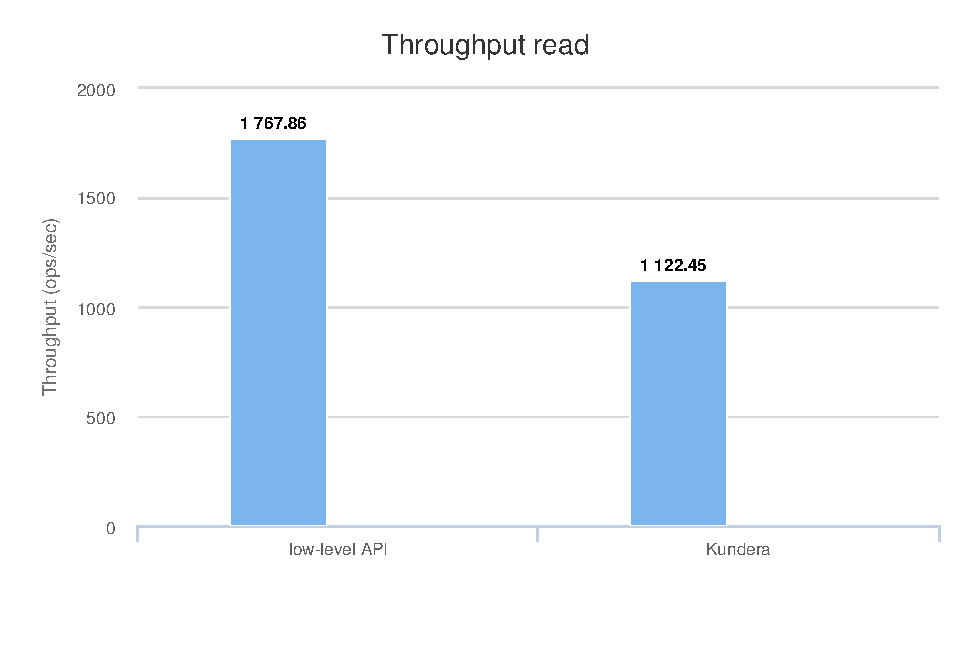
\includegraphics[width=7cm]{images/hbase-read-throughput}
  }
  \subfloat[Latency]{
    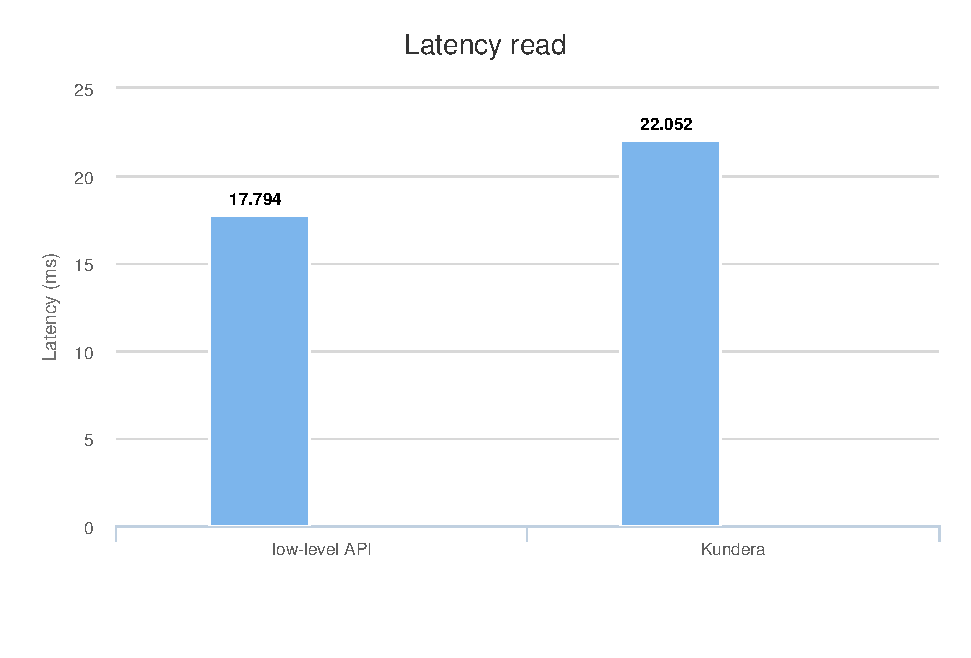
\includegraphics[width=7cm]{images/hbase-read-latency}
  }
  \caption{Hbase - read operation benchmark results}
  \label{fig:hbase-test-read}
\end{figure} 

\begin{figure}[tbh]
  \centering
  \subfloat[Throughput]{
    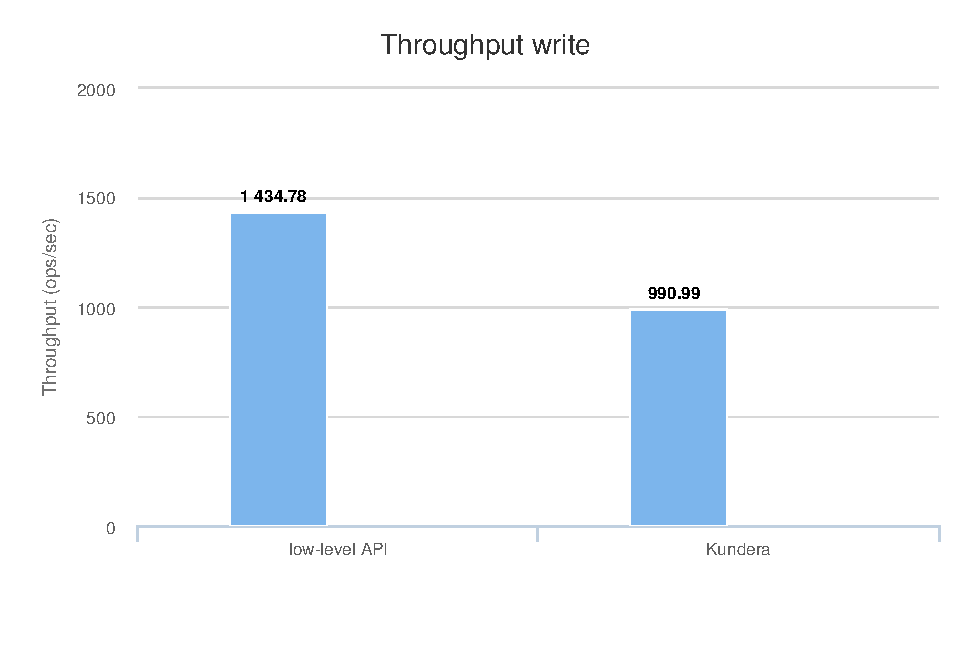
\includegraphics[width=7cm]{images/hbase-write-throughput}
  }
  \subfloat[Latency]{
    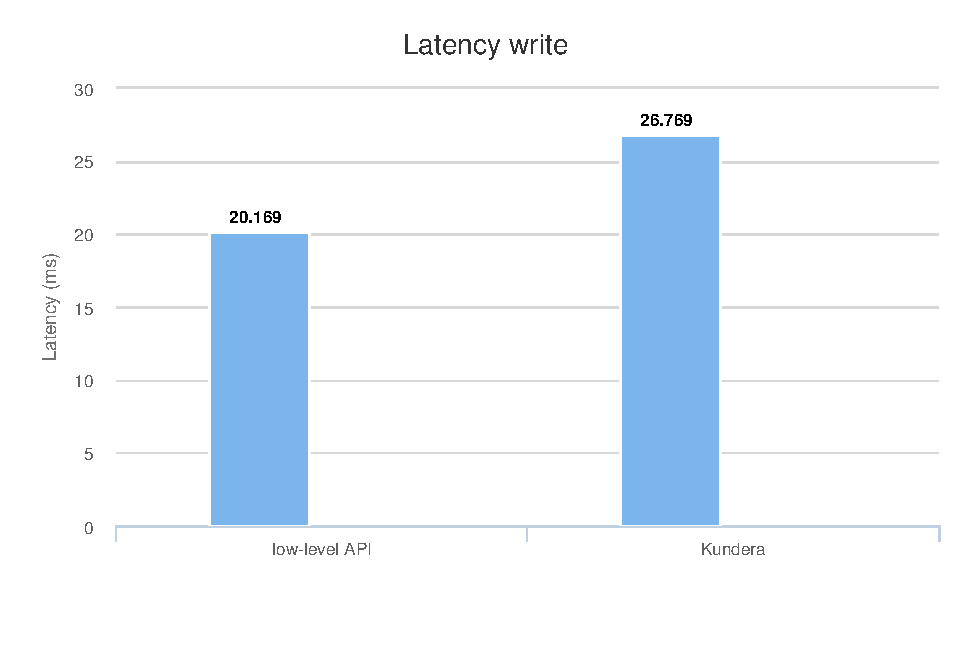
\includegraphics[width=7cm]{images/hbase-write-latency}
  }
  \caption{Hbase - write operation benchmark results}
  \label{fig:hbase-test-write}
\end{figure} 

\subsection{Discussion}
The main objective of our tests was to guarantee that the loss of performance, between the Kundera version of the client and the client written with direct use of the low-level API, was minimum.

\noindent The objective was also to compare our results with the results obtained by Kundera with the other client extensions. Since Kundera executed the tests on databases instance that reside on the testing machine we cannot compare our results, in fact, is meaningless to execute the tests for Google Datastore and Azure Table on the storage emulator installed on a development machine. What we decide to do to has been to test the performance of the newly developed client extensions remotely and thus testing on a real instance of the databases on the cloud but, to be able to compare the results with the Kundera ones, we decided also to replicate the test for Hbase on a instance in the cloud infrastructure of Politecnico di Milano.
Moreover, Kundera tests were quite out-dated since they has been executed on version 2.6 of the clients while as, we write, the latest version is the 2.16.

\newparagraph Apart from the comparison with the Kundera results that cannot be done due to the problem in having a functioning Hbase cluster in the Politecnico di Milano cloud, the tests shows that the performance loss due to the Kundera overhead is minimum or at least acceptable given the advantages that Kundera offer in hiding the NoSQL complexity to the user.
As regards the throughput, can be noticed that the Hbase test done locally over 1.000 entities have a considerably lager value with respect to the throughput of the Google Datastore and Azure Tables tests. This is due to two reasons; the first one is that YCSB benchmarks run until the target database reach saturation and thus tries to estimate the maximum possible throughput, the second reason is due to the fact that, while running remotely, the databases instances are addressed through TCP requests and thus the number of connections that the testing system has to handle becomes the bottleneck. 

\noindent Running the tests with less entities will increase the throughput as the number of connection that needs to be maintained open is significantly lower.
As an evidence of this are reported in figure \ref{fig:gae-1000} and \ref{fig:azure-1000} the results of a test run on the same remote instances but with just 1.000 entities.   

\begin{figure}[tbh]
  \centering
  \subfloat[Write throughput]{
    
\includegraphics[width=5cm]{images/logopm}
  }
  \qquad
  \subfloat[Read throughput]{
    
\includegraphics[width=5cm]{images/logopm}
  }
  \caption{Google Datastore - 1.000 entities benchmark results}
  \label{fig:gae-1000}
\end{figure} 

\begin{figure}[tbh]
  \centering
  \subfloat[Write throughput]{
    
\includegraphics[width=5cm]{images/logopm}
  }
  \qquad
  \subfloat[Read throughput]{
    
\includegraphics[width=5cm]{images/logopm}
  }
  \caption{Azure Tables - 1.000 entities benchmark results}
  \label{fig:azure-1000}
\end{figure} 

\section{Hegira generator}
\label{sec:data}
To be able to test the interaction between the CPIM library and the synchronization system and to provide an example of usage of the extended CPIM library, we have developed \textit{Hegira generator}.

\noindent The application provides two behaviors through command line interface, a \texttt{clean} command to clean-up the remote Datastore instance by deleting all the entities of all Kinds, and a \texttt{generate} command that take as argument the number of entities to be generated per table and generates them.

\newparagraph Data generation is done upon a pre-defined entity model inside the application and described by the ER diagram of figure \ref{fig:hegira-generator-er}.
Build an entity generator agnostic to the entities model was not our goal and it would have required a way to automatically build the dependency graph of the entities since entities related to other ones should have a reference to the entity they depends on. Hence the application is aware of the entities dependencies and generates them accordingly.

\begin{figure}[tbh]
  \centering
  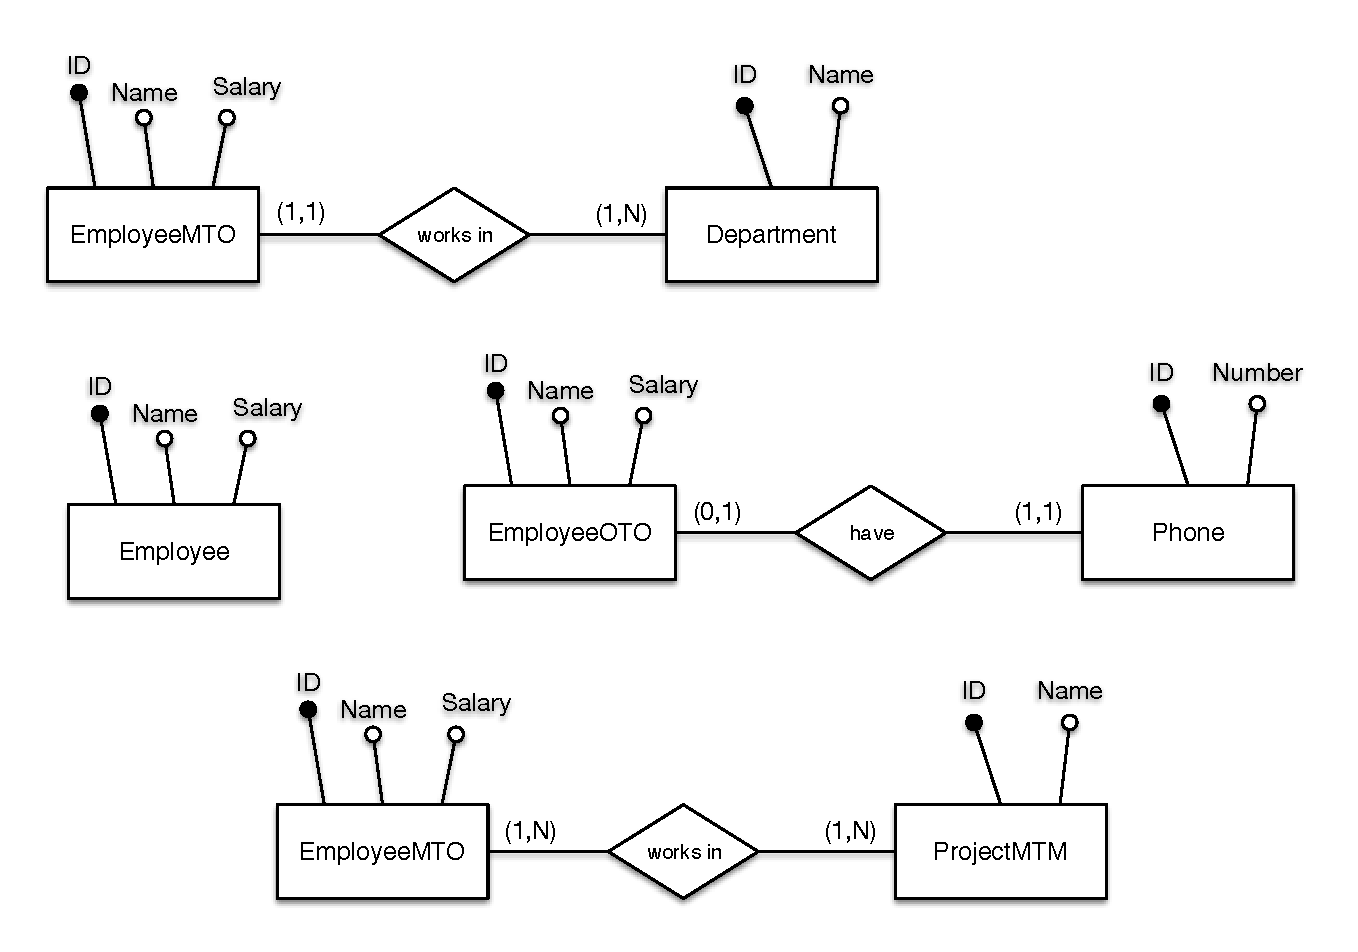
\includegraphics[width=10cm]{images/hegira_generator_er}
  \caption{ER diagram of Hegira-generator model}
  \label{fig:hegira-generator-er}
\end{figure} 

\noindent To be able to generate random entities, two methods are used:
\begin{itemize}
\item \texttt{persist(Class master)} that generates and persist entities without dependencies (such as \texttt{Employee} in the application model;
\item \texttt{persist(Class master, Class slave, DependencyType type)} that generates and persist the entities of the \textit{master} class, then uses randomly extracted entities among those just generated to fill the dependencies for the entities of the \textit{slave} class.
The \texttt{DependencyType} would be \texttt{SINGLE}, if the \textit{slave} class needs just one element to fill the dependency (which is the case of \textit{One to One} and \textit{Many to One} relationships), or \texttt{COLLECTION}, if the \textit{slave} class needs more than one element to fill the dependency (which is the case for \textit{Many to Many} relationships).
\end{itemize}

\noindent The actual entity generation is delegated to the entity itself through reflection since each entity of the model implements the \texttt{Randomizable} interface.
An example of entity genearion through this interface is shown in the snippet \ref{code:randomizable}.

\begin{lstlisting}[language=Java, caption=Entities generation, label=code:randomizable]
@Entity
public class EmployeeOTO implements Randomizable<EmployeeOTO, Phone> {
    ...
    @Override
    public EmployeeOTO randomize(Phone dependency) {
        setName(RandomUtils.randomString());
        setSalary(RandomUtils.randomLong());
        setPhone(dependency);
        return this;
    }
}
\end{lstlisting}
 
\subsection{Exploited CPIM features}
To perform the persist operation of the generated entities is used the \texttt{EntityManager} interface on which is called the \texttt{persist} method, this is completely JPA compliant and the user is not aware of what is done under the hood since communication with the synchronization system is handled automatically. An example is provided in the code \ref{code:example-persist}.

\begin{lstlisting}[language=Java, caption=Persisting entities in CPIM, label=code:example-persist]
CloudEntityManager em = MF.getFactory().getEntityManager();
Department dep = new Department("Computer Science")
em.persist(dep)
\end{lstlisting}

\noindent The persist operation through \texttt{CloudEntityManager} contacts the synchronization system to get the assigned sequence numbers for the specific tables and assign the first of them to the entity before delegating to Kundera the persist operation.

\newparagraph The application make use of the possibility of modifying at run-time the size of sequence numbers range that is requested to the synchronization system. Hence before the persist operation, the size of the sequence number range is set to the double of the number of entities to be generated. This is done through a call to \texttt{SeqNumberProvider.getInstance().setOffset(tableName, offset)}, if the resulting range size is grater than the maximum size that can be requested, is limited to that value. 

\newparagraph the last feature that is exploited by the application is the sequence number backup to file. The backup is configured in the \texttt{migration.xml} file as described in the appendix \ref{app:migration}.
This permit to the application, when is restarted, to restore the sequence numbers without the need of contacting the synchronization system.

\noindent Furthermore, to avoid execution of persist operations on a table which entities generation was completed in a previous execution, a file with the list of the table completely generated is kept in the same folder specified for the sequence numbers backup files.

\section{Summary}
In this chapter we have presented the test of correctness and performance made for the two developed Kundera extension showing the minimal performance loss that Kundera add to the low-level API.
Finally we have presented \textit{Hegira-generator}, the application developed to test the mechanisms developed inside CPIM to interacts with the synchronization system.
